\documentclass[11pt,a4paper]{scrartcl}
%{{{ general stuff
\usepackage[english]{babel}
\usepackage[utf8]{inputenc}
\usepackage[T1]{fontenc}
\usepackage[hidelinks]{hyperref}
\usepackage{float} % use H in figure placement
\pagenumbering{gobble}

%}}}
%{{{ graphics
\usepackage{graphicx} % Bilder
%}}}
%{{{ math
\usepackage{mathrsfs} % mathcal and mathscr
\usepackage{mathtools, amssymb, amsthm}
\usepackage{bm} % cool bold symbols
%}}}

% a todo command===============================================================
\newcounter{todocounter}
\newcommand{\todo}[2][noisnotdefined]{
 \marginpar{\fcolorbox{black}{yellow}{\footnotesize\textbf{todo}}
 \ifthenelse{\equal{#1}{noisnotdefined}}{}{\textcolor{black}{\newline\tiny #1}}}
 \textbf{\ifthenelse{\equal{#2}{.}}
   {\fcolorbox{blue}{white}{\textcolor{blue}{$\maltese$}}}{{\textcolor{blue}{#2}}}}
 \refstepcounter{todocounter}}

%===============================================================================

\date{}

\begin{document}

\section*{Project Proposal for Genetic Algorithms and Evolutionary Programming
by Felix Bartel and D\' avid Kerekes}

We want to apply a genetic algorithm to a neuronal network which is known as neuroevolution.
A big advantage of this scheme is that one only needs an indicator how good the neuronal network is given a certain task.
This can for instance be given by the outcome of a game.
Our game of choice was Blobby Volley 2 which is a simple two-dimensional volleyball game with open source written in C++ with lua support, see Figure \ref{fig:screenshot} (a).

\begin{figure}[H]
\center
\begin{tabular}{cc}
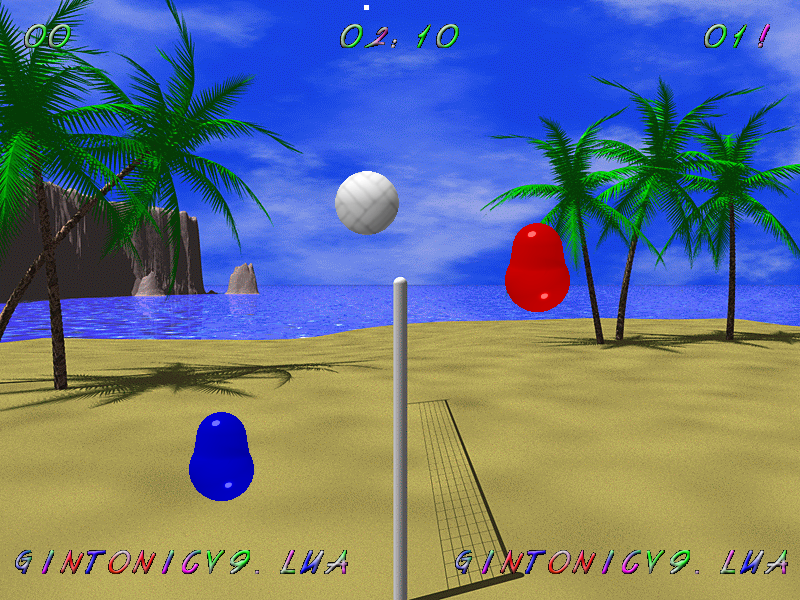
\includegraphics[width=0.3\textwidth]{img/screenshot.png}
&
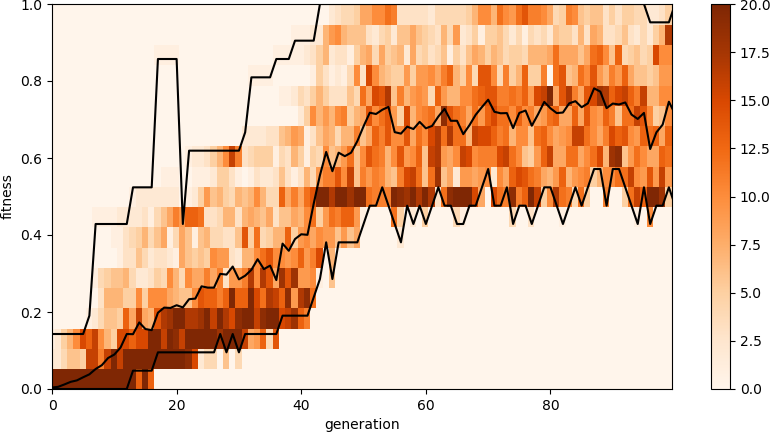
\includegraphics[width=0.4\textwidth]{img/fitness.png}
\\
(a) & (b)
\end{tabular}
\caption{(a) screenshot of the game; (b) fitness density of an example run with indicated minimum, average and maximum}
\label{fig:screenshot}
\end{figure}

A scene from the game could be described by the $x$- and $y$-coordinates of the players and the ball, their corresponding velocities and the current number of ball contacts.
These arguments or a subset of them could then be used as input for the neuronal network.
The output would then be the players movement which only consists of going right, left or jumping.
Assuming the layers of the neuronal network have $n_1,\dots,n_L$ nodes we then have to optimize a function of $\sum_{l=1}^{L-1} (n_l+1)n_{l+1}$ variables if we fix the size of the network.

We have done some tests so far with a basic evolutionary algorithm where we fixed the size of the neuronal network to $6$ input nodes, one hidden layer with $7$ nodes and $2$ output nodes.
As crossover we randomly mixed the weights and biases of two networks and chose the parents via the fitness proportional roulette wheel selection.
Mutation is accomplished by adding Gaussian noise to a subset of the nodes.
Furthermore we implemented elitism.

Because a random neuronal network has barely a change against the given bots in the game, we implemented our own trainer.
The trainer is easier to defeat and even gives up after a certain amount of touches with the ball such that normal gameplay will be rewarded.
This simplification gives the evolutionary algorithm the opportunity to have at least some success rate on which it can hook on.
The results are depicted in Figure \ref{fig:screenshot} (b), where the fitness is the normalized point difference after $21$ serves.

One can see that, although we we made huge simplifications by weakening the opponent, the algorithm produces a network which wins all balls.

We could extend this work by e.g.\,making the size of the network variable or do self-training (maybe with similar techniques as in the paper of Karl Sims which was presented in the lecture)


\end{document}
